%----------------------------------------------------------------------------------------
%	PACKAGES AND OTHER DOCUMENT CONFIGURATIONS
%----------------------------------------------------------------------------------------

\documentclass[12pt]{article}

%%%%%%%%%%%%%%%%%%%%%%%%%%%%%%%%%%%%%%%%%
% Lachaise Assignment
% Structure Specification File
% Version 1.0 (26/6/2018)
%
% This template originates from:
% http://www.LaTeXTemplates.com
%
% Authors:
% Marion Lachaise & François Févotte
% Vel (vel@LaTeXTemplates.com)
%
% License:
% CC BY-NC-SA 3.0 (http://creativecommons.org/licenses/by-nc-sa/3.0/)
% 
%%%%%%%%%%%%%%%%%%%%%%%%%%%%%%%%%%%%%%%%%

%----------------------------------------------------------------------------------------
%	PACKAGES AND OTHER DOCUMENT CONFIGURATIONS
%----------------------------------------------------------------------------------------

\usepackage{amsmath,amsfonts,stmaryrd,amssymb} % Math packages

\usepackage{enumerate} % Custom item numbers for enumerations

\usepackage[linesnumbered, ruled]{algorithm2e} % Algorithms

\usepackage[framemethod=tikz]{mdframed} % Allows defining custom boxed/framed environments

\usepackage{listings} % File listings, with syntax highlighting
\usepackage{setspace}
\usepackage{booktabs}
\usepackage{float}
\usepackage[hidelinks]{hyperref}
\usepackage[normalem]{ulem}

%----------------------------------------------------------------------------------------
%	DOCUMENT MARGINS
%----------------------------------------------------------------------------------------

\usepackage{geometry} % Required for adjusting page dimensions and margins

\geometry{
	paper=a4paper, % Paper size, change to letterpaper for US letter size
	top=2.5cm, % Top margin
	bottom=3cm, % Bottom margin
	left=2.5cm, % Left margin
	right=2.5cm, % Right margin
	headheight=14pt, % Header height
	footskip=1.5cm, % Space from the bottom margin to the baseline of the footer
	headsep=1.2cm, % Space from the top margin to the baseline of the header
	%showframe, % Uncomment to show how the type block is set on the page
}


%----------------------------------------------------------------------------------------
%	NUMBERED QUESTIONS ENVIRONMENT
%----------------------------------------------------------------------------------------

% Usage:
% \begin{question}[optional title]
%	Question contents
% \end{question}

\mdfdefinestyle{question}{
	innertopmargin=1.2\baselineskip,
	innerbottommargin=0.8\baselineskip,
	roundcorner=5pt,
	nobreak,
	singleextra={%
		\draw(P-|O)node[xshift=1em,anchor=west,fill=white,draw,rounded corners=5pt]{%
		\questionTitle};
	},
}


% Define a custom environment for numbered questions
\newenvironment{question}[1][\unskip]{
	\bigskip
	\newcommand{\questionTitle}{~#1}
	\begin{mdframed}[style=question]
}{
	\end{mdframed}
	\medskip
}
 % Include the file specifying the document structure and custom commands

%----------------------------------------------------------------------------------------
%	ASSIGNMENT INFORMATION
%----------------------------------------------------------------------------------------

\title{\textbf{Investigation Into the Influence of Verb Manipulation on Estimated Speed Estimates}} % Title of the assignment

\author{\textbf{Psychology SL Internal Assessment May 2024 Session}\and \textbf{Date of Submission}: 25th October 2023 \and \textbf{Session Number}: 00486-0017\and \textbf{Candidate Code}: kwb492 \and \textbf{Other Group Members' Codes}: kwb583, kwb538, kwb554} % Author name and email address

\date{\textbf{Words}: 2117} % University, school and/or department name(s) and a date

%----------------------------------------------------------------------------------------

\begin{document}

\doublespacing

\maketitle % Print the title
\thispagestyle{empty}
\pagebreak
\tableofcontents
\thispagestyle{empty}

\clearpage
\pagenumbering{arabic}

\pagebreak
\section{Introduction} 
\textbf{Reconstructive memory} is a \textbf{theory} proposed by Bartlett (1932) postulating that memory involves an active process of reconstruction as opposed to passive retrieval. 

Within the theory, two types of information are recognized: information obtained during the perception of an event, and external post-event information. Over time, these two information types are believed to be integrated together, to the point where they seem indistinguishable. Information is believed to be obtained through “fragments” -- small records of pieces of information. During the encoding stage, details may be added to this information to familiarize and better comprehend the information. This links to Bartlett's phrase “effort after meaning,” which indicates how people initially focus on the meaning of an event, then make the effort to interpret the meaning in more familiar terms. When recalling an event, these fragments are recombined, and the gaps filled with past experiences using schemas (cognitive frameworks seeking to organize and categorize information), which may be influenced by social and cultural expectations. Overall, the mentioned characteristics of reconstructive memory suggest memory to be inaccurate and unreliable.  

One study supporting this is Loftus and Palmer's (1974) study, which specifically investigated whether leading questions could change eyewitness memories of an event. In a lab experiment, 45 American university students were allocated to 5 groups, where they were all shown 7 video clips of traffic accidents. After each clip, the participants were instructed to write a brief account of the accident and answer some written questions. This included the leading question (“About how fast were the cars going when they … into each other?”) where the “…” would be replaced with one of 5 manipulated verbs: smashed, collided, bumped, hit, or contacted. From the results, it was found that the range between the lowest (31.8 mph) and highest (40.4 mph) estimated speeds from the groups was 8.6 mph. 

A plausible explanation for the results is that the participants first formed a mental representation of the accident; the verb provided by the integrator then integrated with and altered the participants’ memory according to the verb's severity. This links back to reconstructive memory as the verb (external post-event information) combined with the stored fragments of the accident when recalled, creating a meaningful whole. Furthermore, effort was spent understanding the meaning of the participants' given verbs in relation to the accidents, and then interpreted and integrated into their memories. 

The experiment to be conducted in this investigation is a simplification of Loftus and Palmer’s study; the same leading question will be used, however, as opposed to 5 experimental groups, 2 were decided upon with the manipulated verbs “smashed” and “contacted”. This choice was made based on the results from the original study; the highest and lowest estimated speeds for the verbs demonstrate a clear difference in perceived intensity of the verb. Hence, by selecting the verbs at opposite ends, the aim is to hone in on the difference and the misinformation effect. The original units used (mph) were also changed to km/h to suit a more international participant pool. 

\subsection{Aim}
To investigate whether memory can be altered by misleading post-event information. This is \textbf{relevant} in understanding how memory encoding and recall are influenced, which can in turn influence how police investigators pose their questions to eyewitnesses to minimize memory distortion.  

\subsection{Research Hypothesis (One-tailed)}
The experimental group with the higher intensity manipulated verb (“smashed”) in the leading question will estimate higher speeds (km/h) of a traffic accident collision as opposed to the group with the lower intensity verb (“contacted”). 

\subsection{Null Hypothesis}
There will be no significant difference in speed estimates (km/h) of a traffic accident collision between the experimental group with the higher intensity manipulated verb (“smashed”) in the leading question and the group with the lower intensity verb (“contacted”). 

\subsection{Independent Variable}
Manipulated verb used in the leading question given to the experimental groups: either the higher intensity “smashed,” or lower intensity “contacted.” 

\subsection{Dependent Variable}
Eyewitness memory of the traffic accidents' collision speeds, as operationalized by the speed estimate in km/h. 

\pagebreak
\section{Exploration}
\subsection{Sampling Technique}
To test the aim, participants were chosen using a \textbf{convenience sample} (selecting participants based on their availability and ease of access); tutors for Year 12 students at an international IB English speaking school were contacted for their permission to arrange a time to come in and conduct the experiment. The experiment was conducted with the first tutor that agreed to allow their class to participate in the study. This sample population was chosen as they were 16 or above (able to give consent without a guardian) and had not been exposed to psychological studies, which would have otherwise impacted their responses (demand characteristics). Based on the class arrangements (two students per table, arranged in rows), participants were allocated either of the conditions based on whether they sat on the right or left side of the classroom (split in half). The sampling technique led to 15 and 14 participants in condition A (“smashed”) and condition B (“contacted”) respectively. The total pool of participants was approximately split between males and females (13:16). They shared similar educational and financial backgrounds, representing diverse ethnicities and cultures.  

\subsection{Research Design}
An \textbf{independent measures design} was chosen to test whether the manipulated verb would affect estimated car speed, so each participant was exposed to only one of the conditions. This was chosen as it prevented participants from detecting variations in the leading questions’ verbs, which could have led them to guess the aims of the experiment and express demand characteristics in response. 

\subsection{Controlled Variables}
All the \textbf{instructions, questionnaires (except for verb manipulation), video and procedure were standardized} between conditions (carried out by conducting everything at the same time to maintain control), to limit the effect of confounding variables. \textbf{Maintaining the video choice across both conditions} ensured the variance in estimated car speeds was not due to the change in speeds and setting between the videos (internal validity).  

\subsection{Materials and Procedure}
Two variants of questionnaires [Appendix 3 and 4] were printed and labelled with participant codes for either condition. Both questionnaires contained the same filler questions that would detract attention from the leading question verb (only difference between the variants). 

In line with ethical guidelines, debrief and consent forms were provided. The consent form [Appendix 2] detailed the participants' right to withdraw, which would allow them to have control over their own data. These were also labelled with participant codes and matched to the questionnaires. The debrief [Appendix 6] informed the participants of the study's true aims and allowed for any specific clarifying questions to be asked.  

A PowerPoint presentation was also made to visually maintain the participants' attention, and ensured participants were aware of every step of the procedure and how to carry out the given instructions. 

As for the car crash video (\url{https://www.youtube.com/watch?v=kXaJR-x3ruk}), this was chosen for the clear view of the accident, with identifiable colored cars travelling at approximately similar speeds (ensured that, in the case where the participant estimated the speed of the other involved car, the estimation would not be impacted). 

Finally, the experimental procedure [Appendix 7] was specific in that each researcher was assigned a task and the oral instructions pre-written. This ensured fluidity which minimized participant distraction (due to stuttering, filler words, unpreparedness). 

\pagebreak
\section{Analysis}
\subsection{Descriptive Results}
From the experiment, ratio data was obtained [Appendix 8]. The most appropriate measure of central tendency (\textbf{mean}) and dispersion (\textbf{standard deviation}) for ratio data were chosen and calculated (to find average of speed estimates, how they deviate and to compare them) [Appendix 8]. In the calculated mean scores, condition A's (66.6) was higher than condition B's (41.1). As for the standard deviations, condition A's (“smashed”) (17.2) was higher than condition B's (“contacted”) (25.0). Thus, condition B had a greater spread of scores around the mean score compared to condition A. Therefore, the independent variable (verb manipulation) can be said to have affected the dependent variable (estimated car speed). 

\subsection{Bar Charted Results}
\begin{figure}[H]
	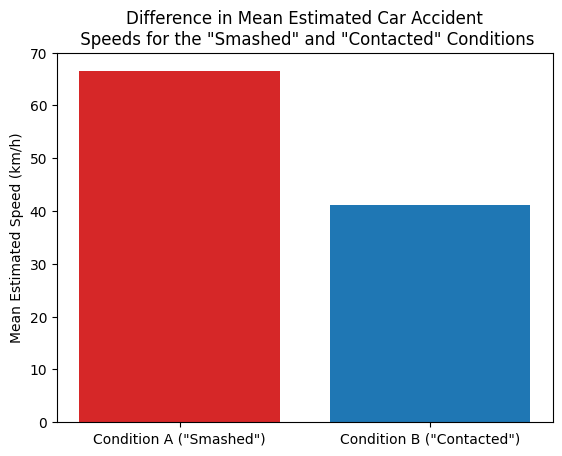
\includegraphics{results}
	\centering
\end{figure}

\subsection{Inferential Results}
Since ratio data was observed and an independent measures design as well as a one-tailed hypothesis was chosen, a Mann-Whitney U-Test was determined to be most appropriate and calculated [Appendix 9] (data was first converted to ordinal as it did not meet requirements for t-test). With 15 participants in condition A and 14 participants in condition B, the critical tabled value [Appendix 10] for significance on a one-tailed test at $p < 0.05$ is 66. The observed U value must be smaller than the tabled value to be significant. The smallest U value chosen was 38.5 which is smaller than 66. Hence, the conclusion is that the null hypothesis is rejected, and the research hypothesis retained. Therefore, the experimental group with the higher intensity manipulated verb (“smashed”) in the leading question did estimate higher speeds (km/h) of a traffic accident collision as opposed to the group with the lower intensity verb (“contacted”). 

\pagebreak
\section{Evaluation}
The two pieces of information recognized by the theory (during event perception, and post event perception) could be identified from the experiment. For the former, this can be observed in how the participants formed a mental representation of the accident during the clip viewing (encoding). The latter is demonstrated by the modified verb in the leading question. It integrated with and altered the participants' memory depending on its intensity. This supports reconstructive memory as the two pieces of information were integrated over time with each other to the point of becoming indistinguishable, which is represented by the higher/lower subconscious answer given (depending on whether they were part of the “smashed” or “contacted” condition). Furthermore, the additional untested questions in the questionnaire supported Bartlett's theory that additional “fragments” are added to make sense of a memory before storing it (effort after meaning). 

One \textbf{advantage} of the chosen experimental design (independent measures) is that it ensured demand characteristics would be limited for participants in the “smashed” and “contacted” conditions, as they would only experience one of the conditions, which eliminated the probability of noticing the verb modifier. A \textbf{disadvantage} of the experimental planning however was in the research method (lab). Although it allowed for a high degree of control over confounding variables, the artificiality of the task (watch car accident clip and complete questionnaire) was unrepresentative of mundane daily tasks and may have led to unnatural responses (low ecological validity). To address this issue, the experimental task can be \textbf{modified} to be conducted in a more realistic, natural setting (casual discussion); within the context of students, they could be asked to engage in a discussion about the video clip instead, with a confederate providing the leading question orally. Although this compromises the degree of control on confounding variables (reducing internal validity), the external validity is increased whilst keeping with ethical guidelines. 

One \textbf{advantage} of the chosen sampling method (convenience) is its low time and monetary cost. This allowed for an overall efficient process in the procedure and data collection (aided with tight time constraints), and reduced researcher bias as the participants were not selectively chosen by us. One \textbf{disadvantage} however is the generalizability of the results to the wider, global population. The participants were students ages 16 to 17 at an international IB school, which represents only a small fraction of the global population. Since most participants also did not have driving experience (underage), their speed estimates may have been skewed. One \textbf{modification} of the study that justifies result generalizability is using a larger more varied sample: having a wider range of ages, ethnicities, education levels, etc. will yield a participant pool that shares more similarities with the global population, and hence a more justified generalization. 

As for the procedure, an \textbf{advantage} would be the standardized instructions, sheets, presentation, etc. across both conditions. This limits the influence of extraneous variables and allows a more confident correlation to be made between the speed estimate and modified verb (independent variable explained by dependent). One \textbf{weakness} of the procedure however is the gender bias in the results due to the condition allocation method. When allocating participants to conditions, the class was split into half, and either side assigned to either condition. Since the majority of participants sat with a member of the same gender, it was noticed that condition B had significantly more female participants whereas A had more males (confounding variable). Although there was a gender bias, this issue can be considered negligeable on the results as speed estimates are not correlated to gender (can be further investigated). Nevertheless, a \textbf{modification} to the experiment to eliminate this issue would be to introduce gender quotas, to ensure an equal number of male and female participants in either condition. 

In conclusion, the results and observations made supported Loftus and Palmer's original study, which reinforces the validity of Bartlett's theory of reconstructive memory. For further investigation, the suggested modifications could be implemented to improve the accuracy and generalizability of the obtained results, or other aspects of the theory can be tested to determine their validity. 

\section{References}
Swash, L. and Sparks, J. (n.d.) \textit{IB Diploma Psychology Core Companion: Cognitive Approach} PDF. tutor2u. Retrieved from \url{www.tutor2u.net/psychology} pp. 42-45 

\section{Appendix}
\subsection*{[1] Instructions}
Good morning, everyone! We thank you for taking the time to participate in this experiment. 

In the experiment you are about to take part in, you will be shown an 11-second clip on the screen at the front of the classroom. After viewing this video, you will be asked to flip over your questionnaire and fill in the questions. You will be given 2 minutes to answer the questionnaire. Please read all the questions carefully. We ask that you answer them all truthfully and to the best of your ability.

During this time and throughout the experiment, please raise your hand if you have any questions and a researcher will do their best to assist you.

A consent form will be given to you. We ask you to read it through and sign your agreement to take part in this experiment. At the bottom, there are a few questions for you to answer regarding your demographics. This information will be kept confidential. Please note that if at any point during the experiment you would not like to participate anymore, you have the right to withdraw your consent and information. From this point onwards, we ask that you remain silent and do not communicate with other participants.

You will now be shown the video.

\textbf{*Video plays*}

\textbf{*Video ends*}

You now have 2 minutes to answer the questionnaire, please flip it over and begin.

\textbf{*2 minutes end*} 

The experiment has ended, please flip over your questionnaire, and do not make any further amendments. Please do not communicate with any other participants until all questionnaires have been collected.

\subsection*{[2] Consent Form}

\begin{figure}[H]
	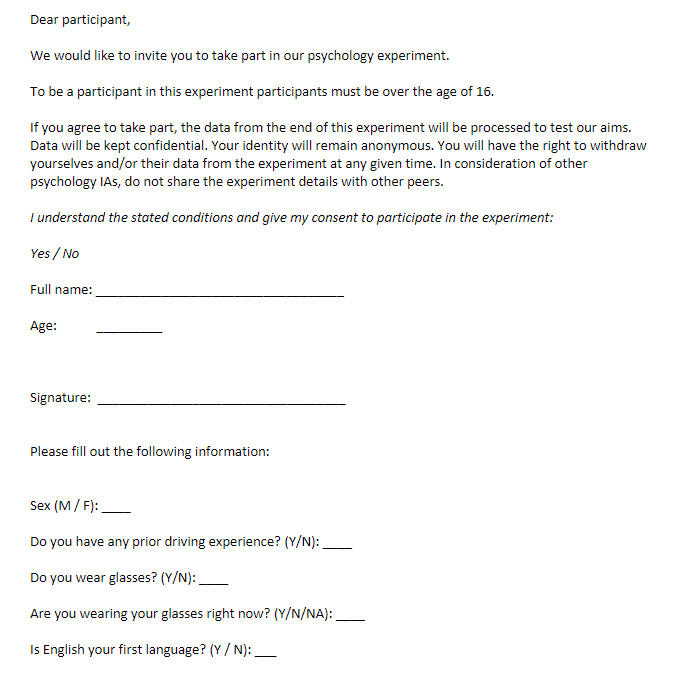
\includegraphics{consent_form}
	\centering
\end{figure}
\pagebreak

\subsection*{[3] Video Clip questionnaire -- Condition A}
\begin{figure}[H]
	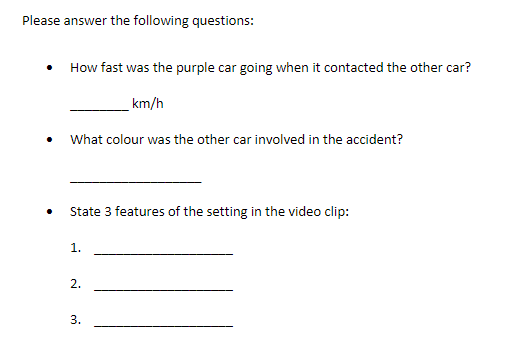
\includegraphics{a_questionnaire}
	\centering
\end{figure}

\subsection*{[4] Video Clip questionnaire -- Condition B}
\begin{figure}[H]
	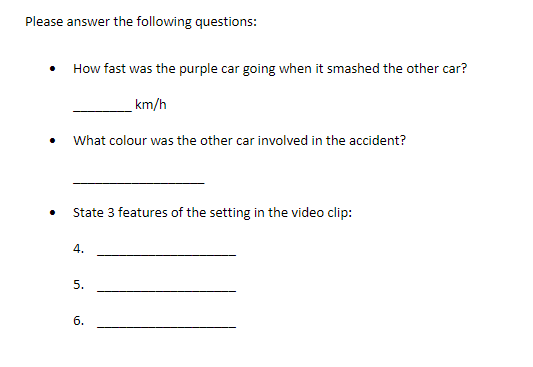
\includegraphics{b_questionnaire}
	\centering
\end{figure}

\subsection*{[5] PowerPoint Presentation}
\begin{figure}[H]
	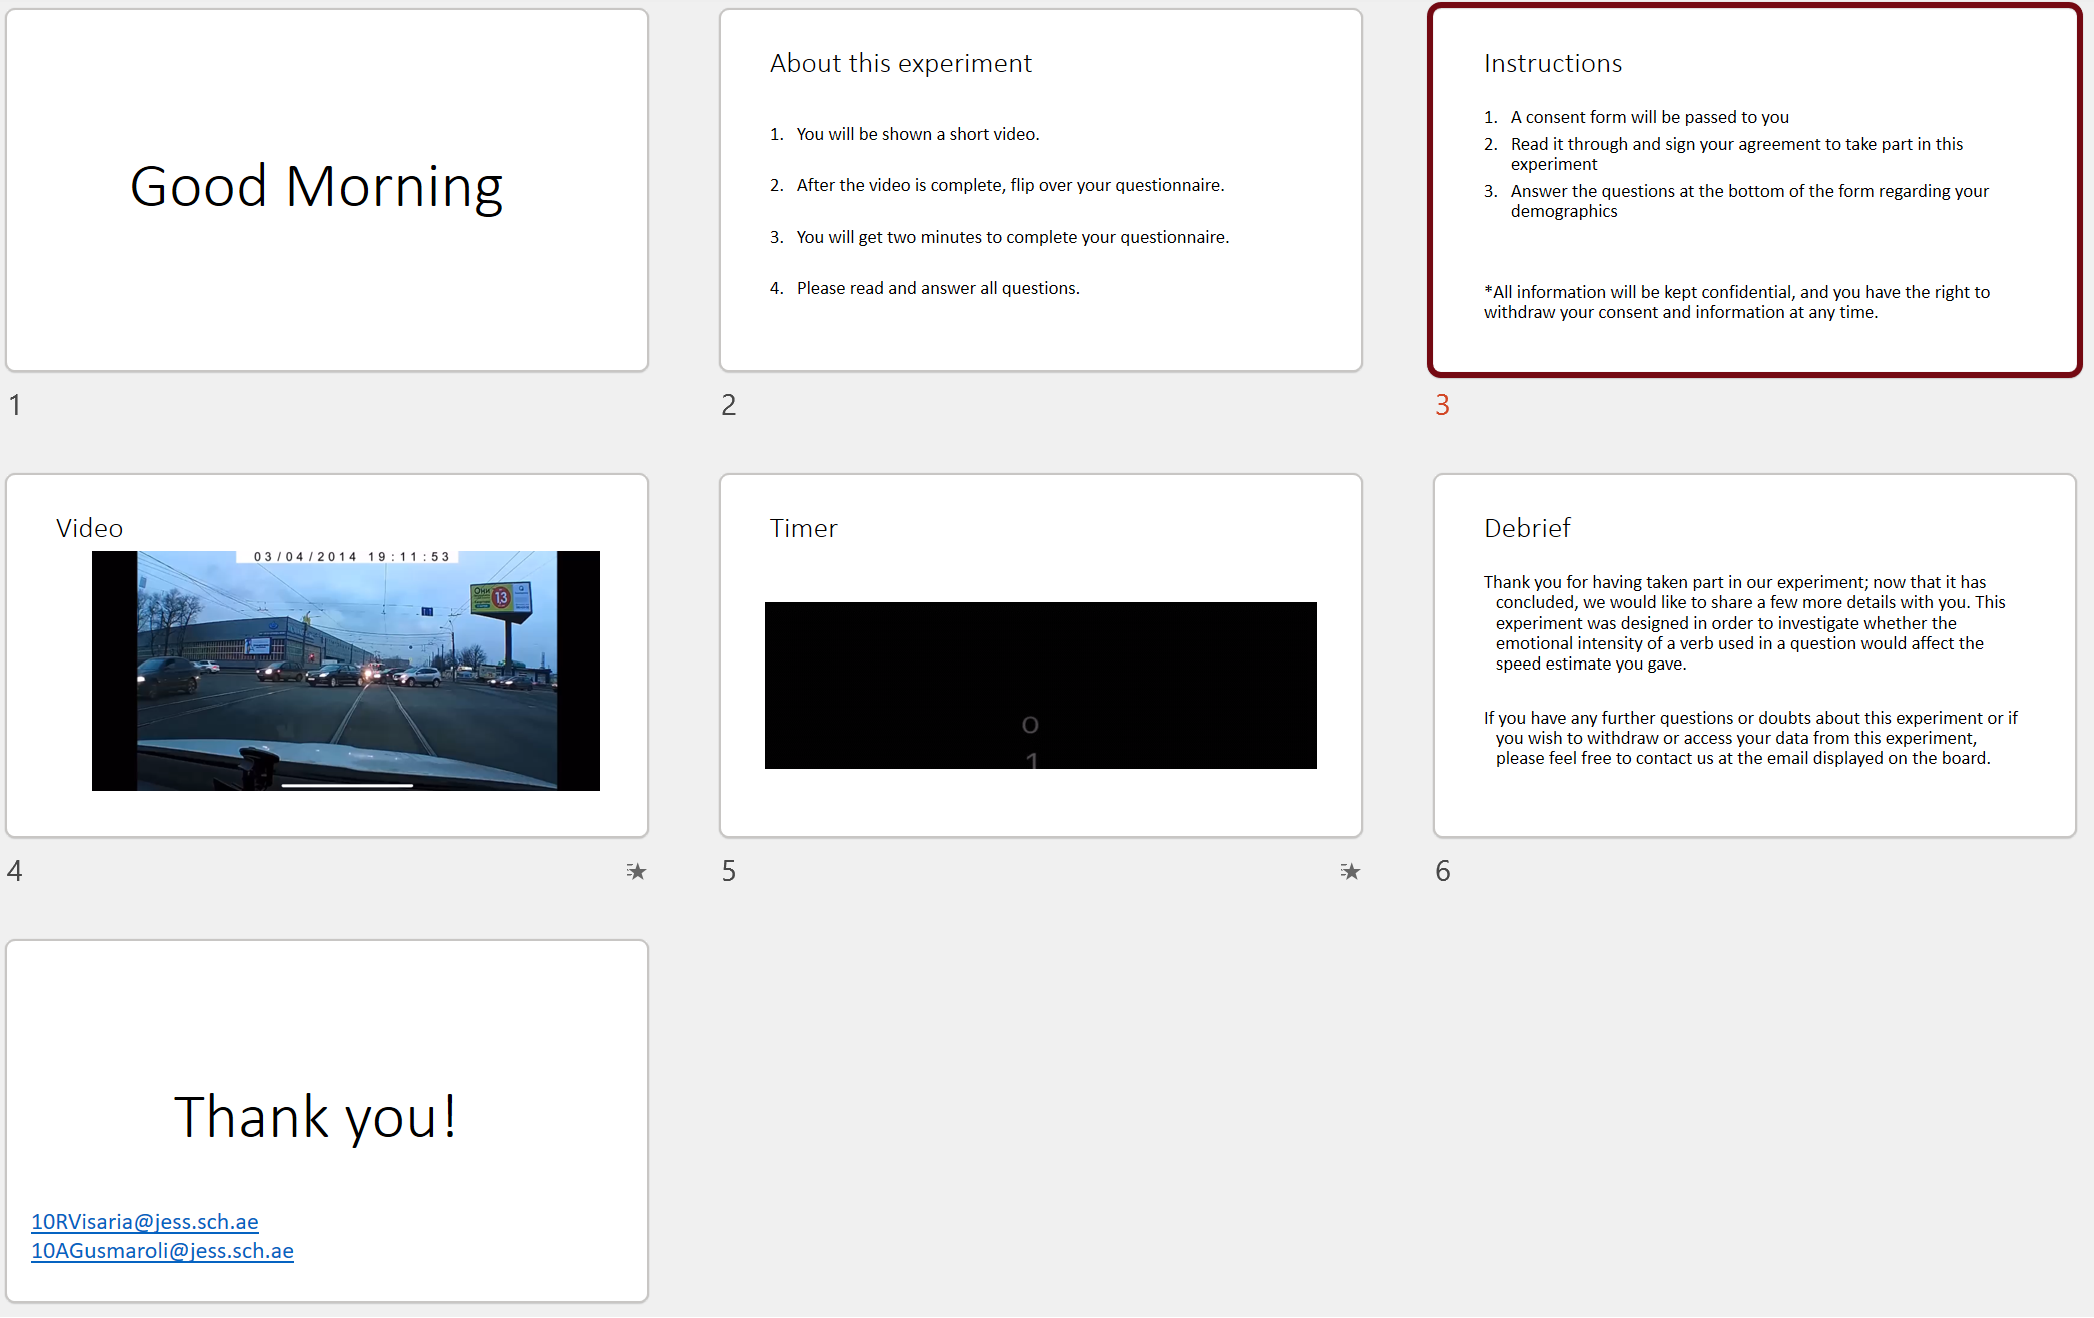
\includegraphics[scale=0.5]{ppt}
	\centering
\end{figure}

\subsection*{[6] Debrief}
Thank you for having taken part in our experiment; now that it has concluded, we would like to share a few more details with you. This experiment was designed to investigate whether the emotional intensity of a verb used in a question would affect the speed estimate you gave.

If you have any further questions or doubts about this experiment or if you wish to withdraw or access your data from this experiment, please feel free to contact us at the email displayed on the board.

\subsection*{[7] Experimental Procedure}
\begin{enumerate}
	\item Researchers entered and informed teacher of experiment commencing.
	\item Researcher A read out instructions while researchers B and C labelled desks with participant codes (A1, A2, B1, B2, etc.).
	\item Researcher B handed out consent forms while researcher D set up presentation (participants meanwhile filled out consent forms). 
	\item Researcher B and C collected consent forms and checked for consent before giving questionnaire with matching participant code.
	\item Second set of instructions read, and video played. 
	\item Participants were given 2 minutes to answer the questionnaire.
	\item Researchers B and C collected completed questionnaires while researcher D read debrief. 
\end{enumerate}

\subsection*{[8] Results Table}
\begin{figure}[H]
	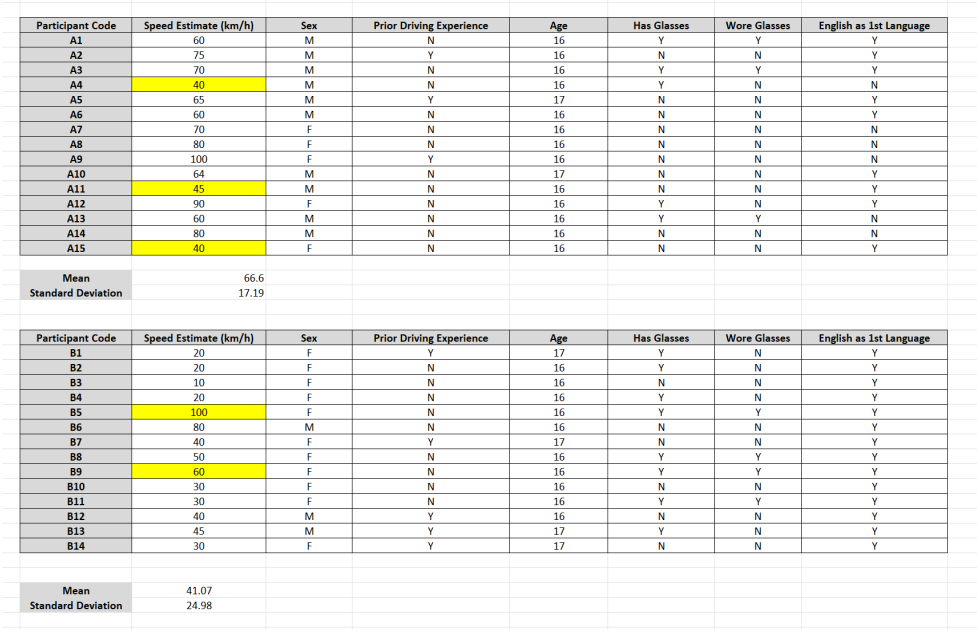
\includegraphics[scale=0.8]{results_table}
	\centering
\end{figure}

\subsection*{[9] Mann Whitney U-Test}
\begin{figure}[H]
	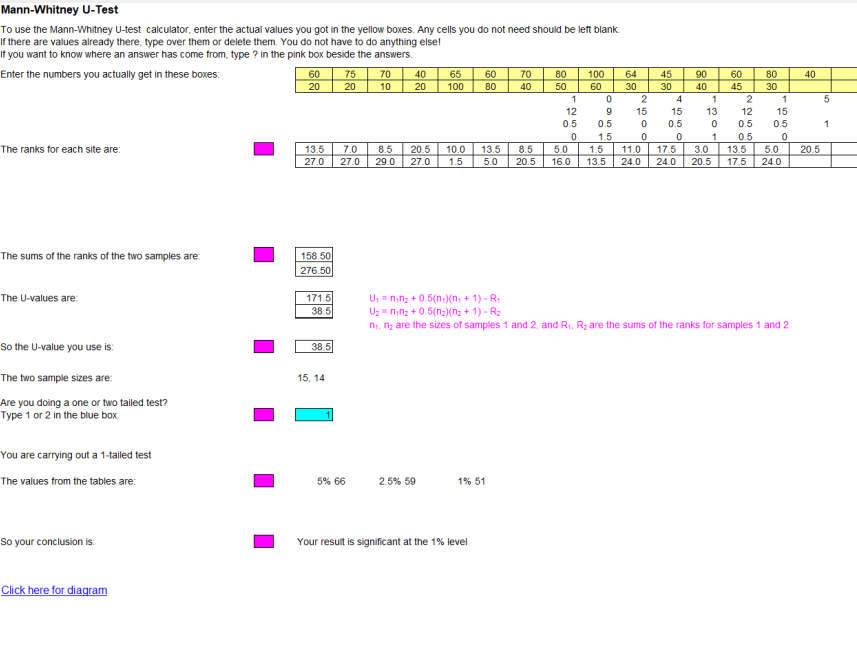
\includegraphics[scale=0.9]{mann-test}
	\centering
\end{figure}

\subsection*{[10] Critical Values Table}
\begin{figure}[H]
	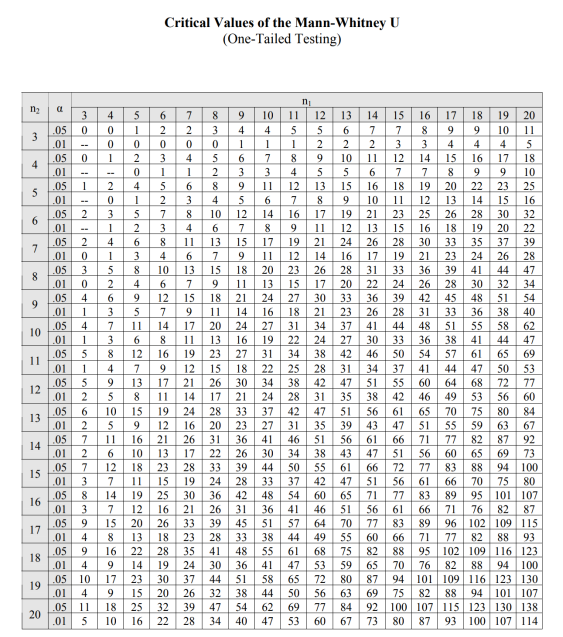
\includegraphics{crit-values}
	\centering
\end{figure}

\end{document}
